%\subsection{\nexp\ Strategy}

Precision frontier experiments require very high statistics as well as extensive evaluation of systematic uncertainties, backgrounds, biases and distortions in the data selection criteria. The two most recent pion decay experiments, TRIUMF PIENU and PSI PEN  provide highly insightful information on the  limitations of their techniques and the principal systematic effects which we have incorporated into our design concepts discussed below. These  measurements were performed using stopped pions that decay at rest either directly to a positron and a neutrino ($\pi^+ \rightarrow e^+ \nu$ decay) or first to a muon (and associated neutrino) that subsequently undergoes 3-body decay at rest in the target (decay chain $\pi^+ \rightarrow \mu^+ \rightarrow e^+$).  The  energy and time characteristics of the positrons emerging from those two decays are very different, and thus can be used to distinguish the decay channels. By measuring the ratio of positrons detected from the two channels, many systematic effects (e.g. pion counting, solid angle acceptance, efficiency, etc.) cancel out to first order, aiding in reaching high precision.  Despite being  mono-energetic the positrons originating from $\pi^+ \rightarrow e^+ \nu$ decays have their energy distribution broadened due to finite energy resolution of the calorimeter, shower leakages of low energy photons from the sides and ends of the calorimeter as well as the presence of radiative decays. Those effects result in a low energy tail hidden under the Michel spectrum and lead to the main correction and largest source of systematic effects in the branching ratio measurement. In order to minimize the energy tail for a precise experiment, a high resolution,  high radiation-length, and high acceptance calorimeter must be chosen.  Other significant systematic effects are associated with pulse pile-up and decays-in-flight of pions prior to stopping in the target. To supress all these  small effects to the level $< 0.01\%$ we propose to use a highly segmented stopping target.

The new measurement of $R_{e/\mu}$ would build on the techniques refined in the previous
experiments with high energy resolution like TRIUMF PIENU and high acceptance for positrons and
gammas like PSI PEN. In addition, it would employ emerging technologies in 
highly granular 4-dimensional tracking in an active stopping target using low gain avalanche 
diode (LGAD) silicon detectors. The combination of these two features, tracking in a highly
segmented fast active target (ATAR) and a high acceptance fast electromagnetic calorimeter (CALO) promise
to reduce the systematic impact of key challenges in the earlier experiments.

In the following we focus on the $R_{e/\mu}$ aspect of the proposed program because the systematic
requirements for achieving O$(10^{-4})$ precision are very demanding. The pion beta decay experiment
would equally benefit from the fast response of both active target and calorimeter, but the 
target thickness will be increased to spread out the wider stopping range of the 
%foreseen $\sim$100 MeV/c
pion beam with 100-fold higher rate than required for the $\pi \rightarrow e(\mu)$ measurement. 


%\subsection{Statistics}

%It is estimated that $3 \times 10^8\; \pi^+ \rightarrow e^+ \nu$ %events can be collected in two years of operation, satisfying the %statistics goal. 

%In addition to improvements in the precision of the PIENU branching ratio, orders of magnitude improvements would be anticipated in sensitivity to sterile neutrinos in decays $\pi^+ \rightarrow e^+/\mu^+ \nu_H$ and to decays involving dark sector particles like $\pi^+ \rightarrow e^+/\mu^+ \nu \textrm{X}$ as mentioned in Sec. \ref{Exotics}.

%\todo{Statement for PiBeta}


\subsection{Active Target (ATAR)}
\begin{figure}[h!]
\centering
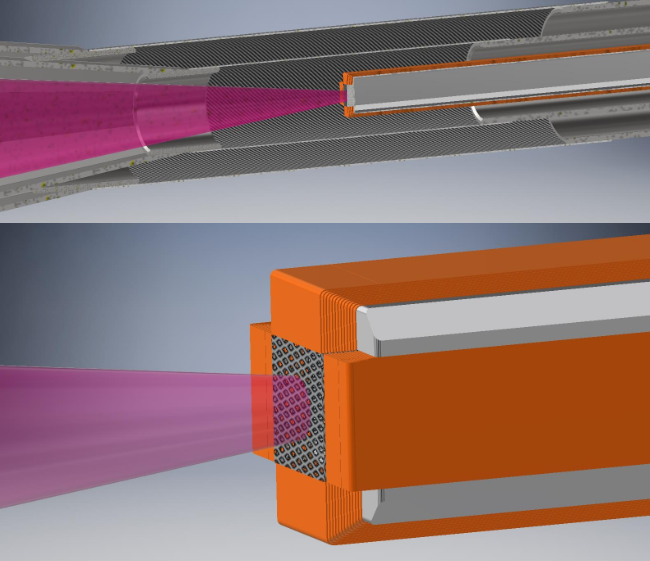
\includegraphics[scale=0.4]{sections/figures/atar1.png}
\caption{place holder: fig:atar1}
\label{fig:atar1}
\end{figure}

Fig.~\ref{fig:atar1} shows a concept drawing for  the pion beam entrance channel and  the active target. The  focused and collimated beam with a 1 cm diameter area passes through degrading plastic scintillators and two layers of double sided Si-strip detectors (not shown) before hitting the target. 
The stopping target (ATAR) is a rectangular prism of 20 mm transverse size and 5.76 mm in beam direction. It consists of 48 layers of AC LGAD sensors with a strip pitch of 200 $\mu m$. This results in 100 channels per layer and 4800 channels for the full detector. Consecutive layers are rotated by 90 degrees.

%Before describing the target (ATAR) in detail, let us recall its The target has the following functionalities:


\begin{itemize} 
\item 
Pion stops are identified. The expected stopping distributions are presented in fig.~\ref{fig:sim.stops}.
\begin{figure}[h!]
\centering

\includegraphics[scale=0.4]{sections/figures/ph.png}
\caption{place holder: fig:sim.stops}
\label{fig:sim.stops}
\end{figure}

\item
The $\pi \rightarrow \mu \rightarrow e$ Michel chain has to be suppressed by several orders of magnitude for measurement of the calorimeter energy response tail. The expected temporal pulse pair resolution of $dt\sim$1 ns provides a suppression factor of $\lambda_\pi dt=0.038$. An additional suppression results from a tight observation window of 
%several 
about one
pion lifetime, which disfavors the slower muon decay. Further separation is based on topology and energy 
deposition. Muons from pion decay have 4.1 MeV energy and a projected range of 0.8 mm in silicon. The $<$200 $\mu m$ segmentation of the detector was
chosen to resolve most tracks of isotropically emitted muons (see section~\ref{sec:simulation}). A zig-zag strip pattern will identify
the small fraction of muon tracks which stay within a layer and parallel to a strip. Fully depleted silicon detectors with minimal dead material
are essential to fully utilize the energy information. The required dynamic range of the readout is large as a pion can deposit 2 MeV in a
200 $\mu m$ range compared to 40 keV for a MIPS. \todo{MIPS number correct? Simone}

\item 
The "old" muons, accidental muons stops preceding the trigger signal, were a significant background in the previous generation of experiments by generating additional components in the time distributions
presented in fig.~\ref{fig:T1A}. In the PIENU experiment those were kept at an acceptable level, by imposing a wide pile-up window to -7 $\mu s$ before
the pion stop to let old muons decay, at the cost of 60\% of the statistics. For \nexp\, with its 
%5$\times$ 
higher beam rate, this is not 
%an option.
desirable.
Moreover the accidental rate will increase according to the increase of the beam rate. The much faster calorimeter will significantly reduce the pile-up contributions, which are more difficult to model and to determine correctly. In addition we will study how to reduce these accidentals by developing a local pileup rejection approach,
i.e. checking whether the observed decay electron belongs to the stopping vertex of the triggering pion.

\item
Muons arising from upstream pion decays are  relatively easily identified 
by their energy loss dE/dx properties and by  
kinks in their trajectories.
Pion decay
inside the target will be separated by kinks in the topology, dE/dx along the track, c.f. section~\ref{sec:simulation}, and range in the target. A sufficient Michel chain suppression and the tail suppression afforded by the 
%hermetic 
large acceptance
CALO will also allow  constraining a subtle background from Michel decays where the 4.1 MeV
 muon decays before leaving a track in the ATAR. 

\item
The ATAR will also be essential in defining event triggers. As will be discussed in section~\ref{section:daq}, the triggers will include
a relative simple CALO trigger based on all events above the Michel edge. An additional selective trigger based on fast ATAR tracking should suppress the $\pi-\mu-e$ sequence
to such extent, that the fully digitized ATAR information can be stored. The ultimate goal of this analysis is the offline suppression of Michel events so that the
low energy tail of the $\pi \rightarrow e \nu$ response can be measured in-situ. 

\end{itemize}



\todo{ATAR concept by Simone and Abe, please also sketch the readout. Need to address charge sharing. Peter sketched the ATAR readout in the DAQ section, as a starting point for Lawrence and Tim} 

While the LGAD ATAR design is the baseline option, we will also study a scintillating fiber option. Crossed planes of 250 $\mu m$ diameter
fibers should work well with the large signals expected. Recent developments in ultrafast fibers based on a new type of high performance nanostructured organosilicon luminophores (Kuraray NOL-11) and the  multi-channel  SiPM  array from  Hamamatsu  HPK  (S13552-HRQ) built for LHCb provide promising hardware components for this alternative.


\subsection{Calorimeter (CALO)}
\begin{figure}[h!]
\centering
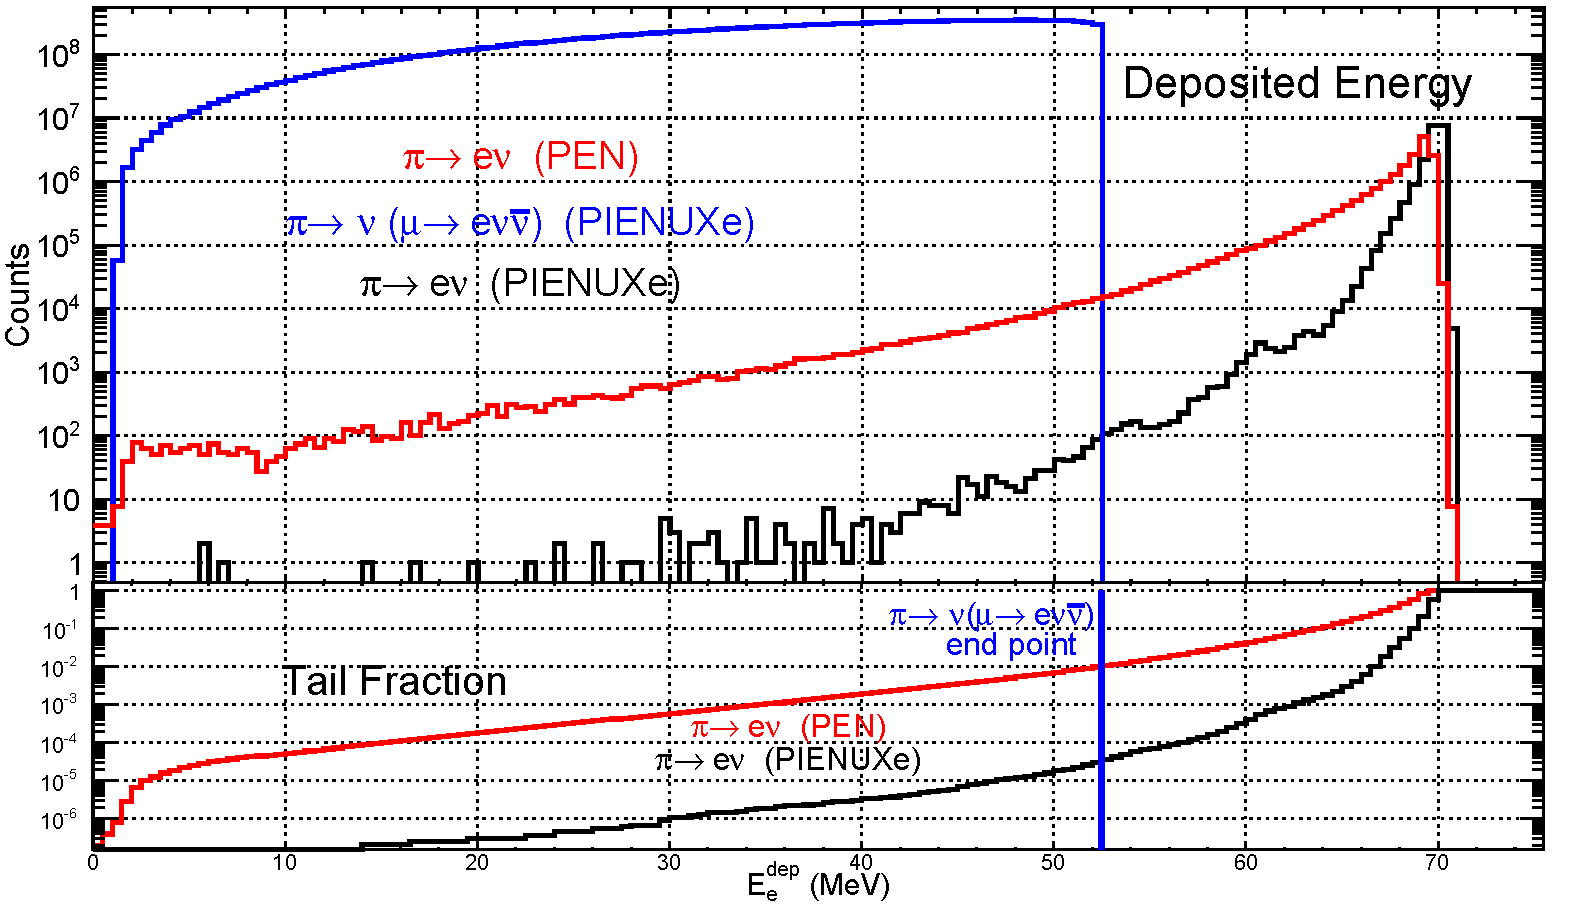
\includegraphics[scale=0.6]{sections/figures/tail.png}
\caption{Upper plot: histogram of $E_{e}^{dep}$, the $\pi_{e2}$ positron energy deposited in active components for a proposed 28 $X_{0}$ thick spherical LXe concept detector (black), compared with the same for the 12 $X_{0}$ pure CsI PEN apparatus (red), along with energy deposition
for the background $\pi \rightarrow \mu \rightarrow e$ decay chain events (blue).  Lower plot: comparison of the corresponding "tail" fractions as a function of $E_{e}^{dep}$; the LXe concept detector improves on the PEN fraction by two orders of magnitude in the region of interest.
\todo{I think we should add a PIENU spectrum as well and change the text accordingly}}
\label{fig:tail}
\end{figure}


A calorimeter covering 3$\pi$ solid angle with a thickness of 28 $X_0$ could dramatically reduce the ``tail” region
%-of-interest, 
which overlaps with the Michel spectrum, a key source of systematic uncertainty, see fig.\cite{fig:tail}. 
Two scintillation calorimeter options are presently under consideration: Liquid xenon and LSO crystals. Their main properties are compared in 
Table~\ref{tab:calos}. Evaluations  of potential energy and timing performance, rate capabilities, mechanical and cryogenic facilities, and cost are ongoing.
\begin{table}
\center
\begin{tabular}{cccccccc}
\hline
\hline
 detector 	&  density 		& 	dE/dx	&	$X_0$ 	& 	$R_M$ 	& decay time 	& $\lambda_{max}$ 	& light output  \\
 			&	g/cm3		&	MeV/cm	&	cm		&	cm		&	ns			&	nm				&	\%		\\	
\hline
LXe			&	2.953 		&	3.707	&	2.872	&	5.224	&	3, 27, 45	&	178			&	125 ?  \\
LSO(Ce)		&	7.40			&	9.6		&	1.14	&	2.07	&	40		&	402			&	85		\\	
\hline
\hline
\end{tabular}
\caption{LXe and LSO properties: density, minimum ioization, radiation length, Moli\`ere radius, decay times, maximum emission wavelength and relative light output compared to NaI(Tl). The LXe boiling point at 1 atm is 165.1 K. \todo{please check, LXe light output?}}
\label{tab:calos}
\end{table}


\subsubsection{LXe Calorimenter}
\begin{figure}[h!]
\centering
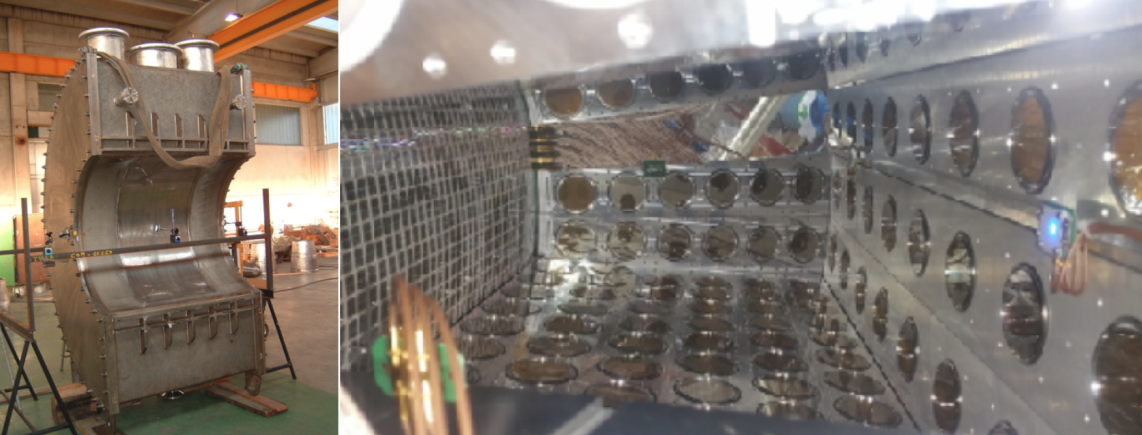
\includegraphics[scale=.4]{sections/figures/calo.meg.png}\vspace{3mm}\\
\caption{placeholder MEG, Toshiyuki please provide nice pictures}
\label{fig:calo.meg}
\end{figure}

One  concept for the new experiment is based on a liquid xenon (LXe) scintillating calorimeter for detection of positrons and gammas from pion decays. A 25-30 X$_o$ thick LXe scintillation calorimeter read out with fast-digitized SiPMs
has extraordinary properties including high light output (65k photons per MeV deposit), fast timing
($\sim$ ns decay time), and near complete containment of EM showers, making it suitable for this
application. Based on experience with the MEG LXe photon calorimeter \cite{Baldini} (see fig.~\cite{fig:calo.meg}) it is reasonable to
expect 1-2 \% energy resolution (comparable to \cite{Aguilar-Arevalo3} ), 50 ps timing resolution, and transverse (depth) position resolution of 5 mm 
(6 mm). Our Japanese collaborators are world experts on this detector technology. They have established basic LXe properties and suitable
simulation codes, conditioned on the MEG detector response, which will be critical for scaling up the design. \todo{Toshiyuki, Toshi, Sathoshi, that's just a placeholder for your part}
Due to the fast scintillation response of LXe (orders of magnitude faster than the NaI(Tl) and
pure CsI used in \cite{Aguilar-Arevalo1, Aguilar-Arevalo2} and \cite{Pocanic1, Pocanic2}), a low-energy pion beam rate of several 10$^5$ Hz can be used, more than an order of magnitude greater than previous experiments, which were impacted by pulse pile-up effects. Systematic effects would be reduced due to the highly uniform response and depth of the total absorption LXe calorimeter. 

\begin{figure}[h!]
\centering
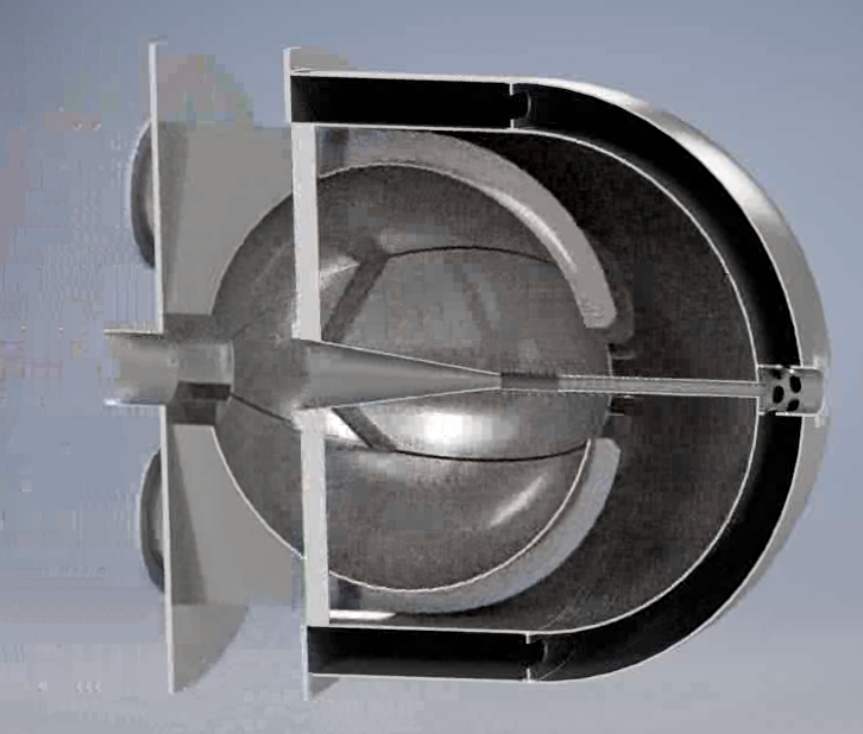
\includegraphics[scale=.4]{sections/figures/calo.Xe.png}
\caption{placeholder  \nexp\ CALO }
\label{fig:calo.Xe}
\end{figure}

\begin{table}
\center
\begin{tabular}{llll}
\hline
\hline
 parameter  &  	value		& 	unit		&  comment \\
\hline
Xe shell radius				&		&		&		\\
Xe volume					&		&		&		\\
Xe weight					&		&		&		\\
Xe entrance window radius	&		&		&		\\
vacuum window radius		&		&		&		\\
\hline
SiPM sensor size			&		&		&		\\
\# sensors					&		&		&		\\
\hline
\hline
\end{tabular}
\caption{Basic \nexp\ CALO parameters. \todo{Xe Ryan, SiPM Toshi, Satoshi et al}}
\label{tab:detpar}
\end{table}
The current conceptional design of the \nexp\ CALO draws on the experience of MEG, but involves several new features, see fig.~\ref{fig:calo.Xe} and Table~\ref{tab:detpar}.
\todo{Ryan: please continue}




\subsubsection{Crystal Calorimeter}


Another calorimeter concept is based on using LSO or LYSO crystals in a $3 \pi$ solid angle configuration similar to the PEN experiment discussed above. LSO has similar timing parameters to pure CsI (fast component aobut 45 ns) but much higher ligt output i.e. 75$\%$ of NaI(Tl). With a short radiation lenght about 1.1 cm, a compact calorimeter of 25-30 $X_0$ with excellent energy and time resolutions could be constructed. The same energy tail suppression would be realized as discussed above for the LXe option. The potential advantages of the crystal calorimeter approach include the absence of cryogenics and dead material, simpler mechanical facilities, and natural segmentation for handling high rates.

\subsection{Tracking}
\input {sections/Detector/tracking.tex}
\subsection{DAQ}
\input {sections/Detector/daq.tex}
\subsection{Simulations}
\label{sec:simulation}

\begin{figure}[h!]
\centering
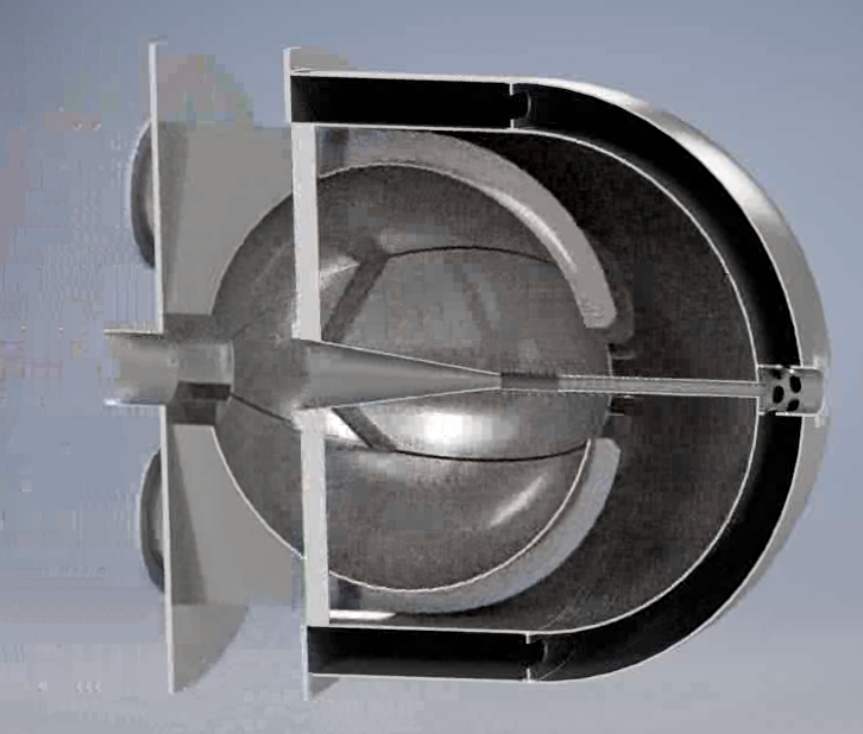
\includegraphics[width=.4\textwidth]{sections/figures/calo.Xe.png}
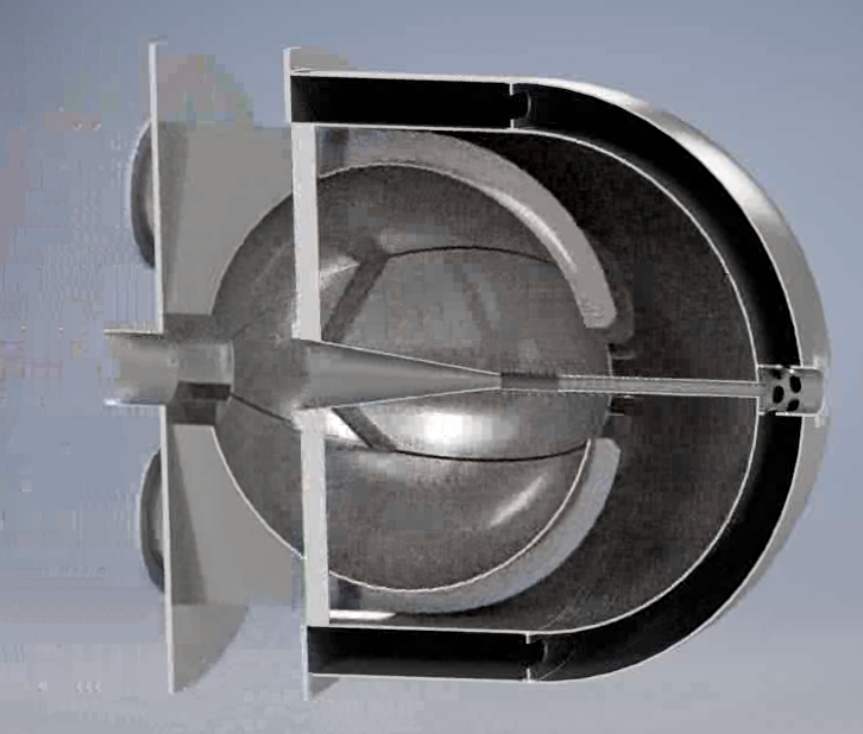
\includegraphics[width=.4\textwidth]{sections/figures/calo.Xe.png}
\caption{Left: A view of the active target system, showing the alternating planes. Right: A view of the full simulation,showing the calo }
\label{fig:simulation.view}
\end{figure}

A Monte Carlo simulation of the ATAR and CALO systems, based on the Geant4 simulation toolkit \cite{geant4}, has been undertaken in recent weeks. The simulated ATAR consists of 50 planes of 100 silicon strips, with the orientation of the strips within each plane rotated 90$^\circ$ with respect to its neighbours. Each strip has a $200 \mu m$ pitch and $120 \mu m$ thickness, giving our target an overall size of $20 mm \times 20 mm \times 6 mm$. Each strip can be read out separately in the simulation, allowing us to track particles as they move and decay within the target. A pure $\pi^{+}$ beam with a momentum spread of $72.84MeV \pm 0.01023$\% is situated upstream of the target. A degrader consisting of plastic scintillator is situated immediately upstream of the target, and its thickness of $7.5 mm$ was tuned such that beam pions are stopped in the center of the ATAR. Surrounding the ATAR and degrader is a carbon fiber beampipe, which acts as a low-Z window for positrons entering the CALO volume. The simulated volume of the CALO system consists of a $80 cm$ LXe sphere with a $17^{\circ}$ cone removed upstream of the ATAR for beam focusing and a $5 cm$ cylindrical cutout for the target and beampipe. Energy deposited in the CALO can be read out both through Geant4 truth information and by counting the scintillation photons which reach the outer radius of the detector.

Because of the lack of dead volume within the ATAR, as we can expect for AC-LGADs of this thickness, each particle leaves a distinctive track and energy signature. These signatures are not only useful for tagging decays of interest, but also supress our most common sources of background: decays in flight.